% in this file I leave the figure captions outside\ caption{} because I want them
to be formatted in the same way as the general text (double spaced and linenumbered)
\captionsetup[figure]{labelfont={sc},labelformat={default},labelsep=period,name={Figure}}

\newpage
\begin{figure}[!h]
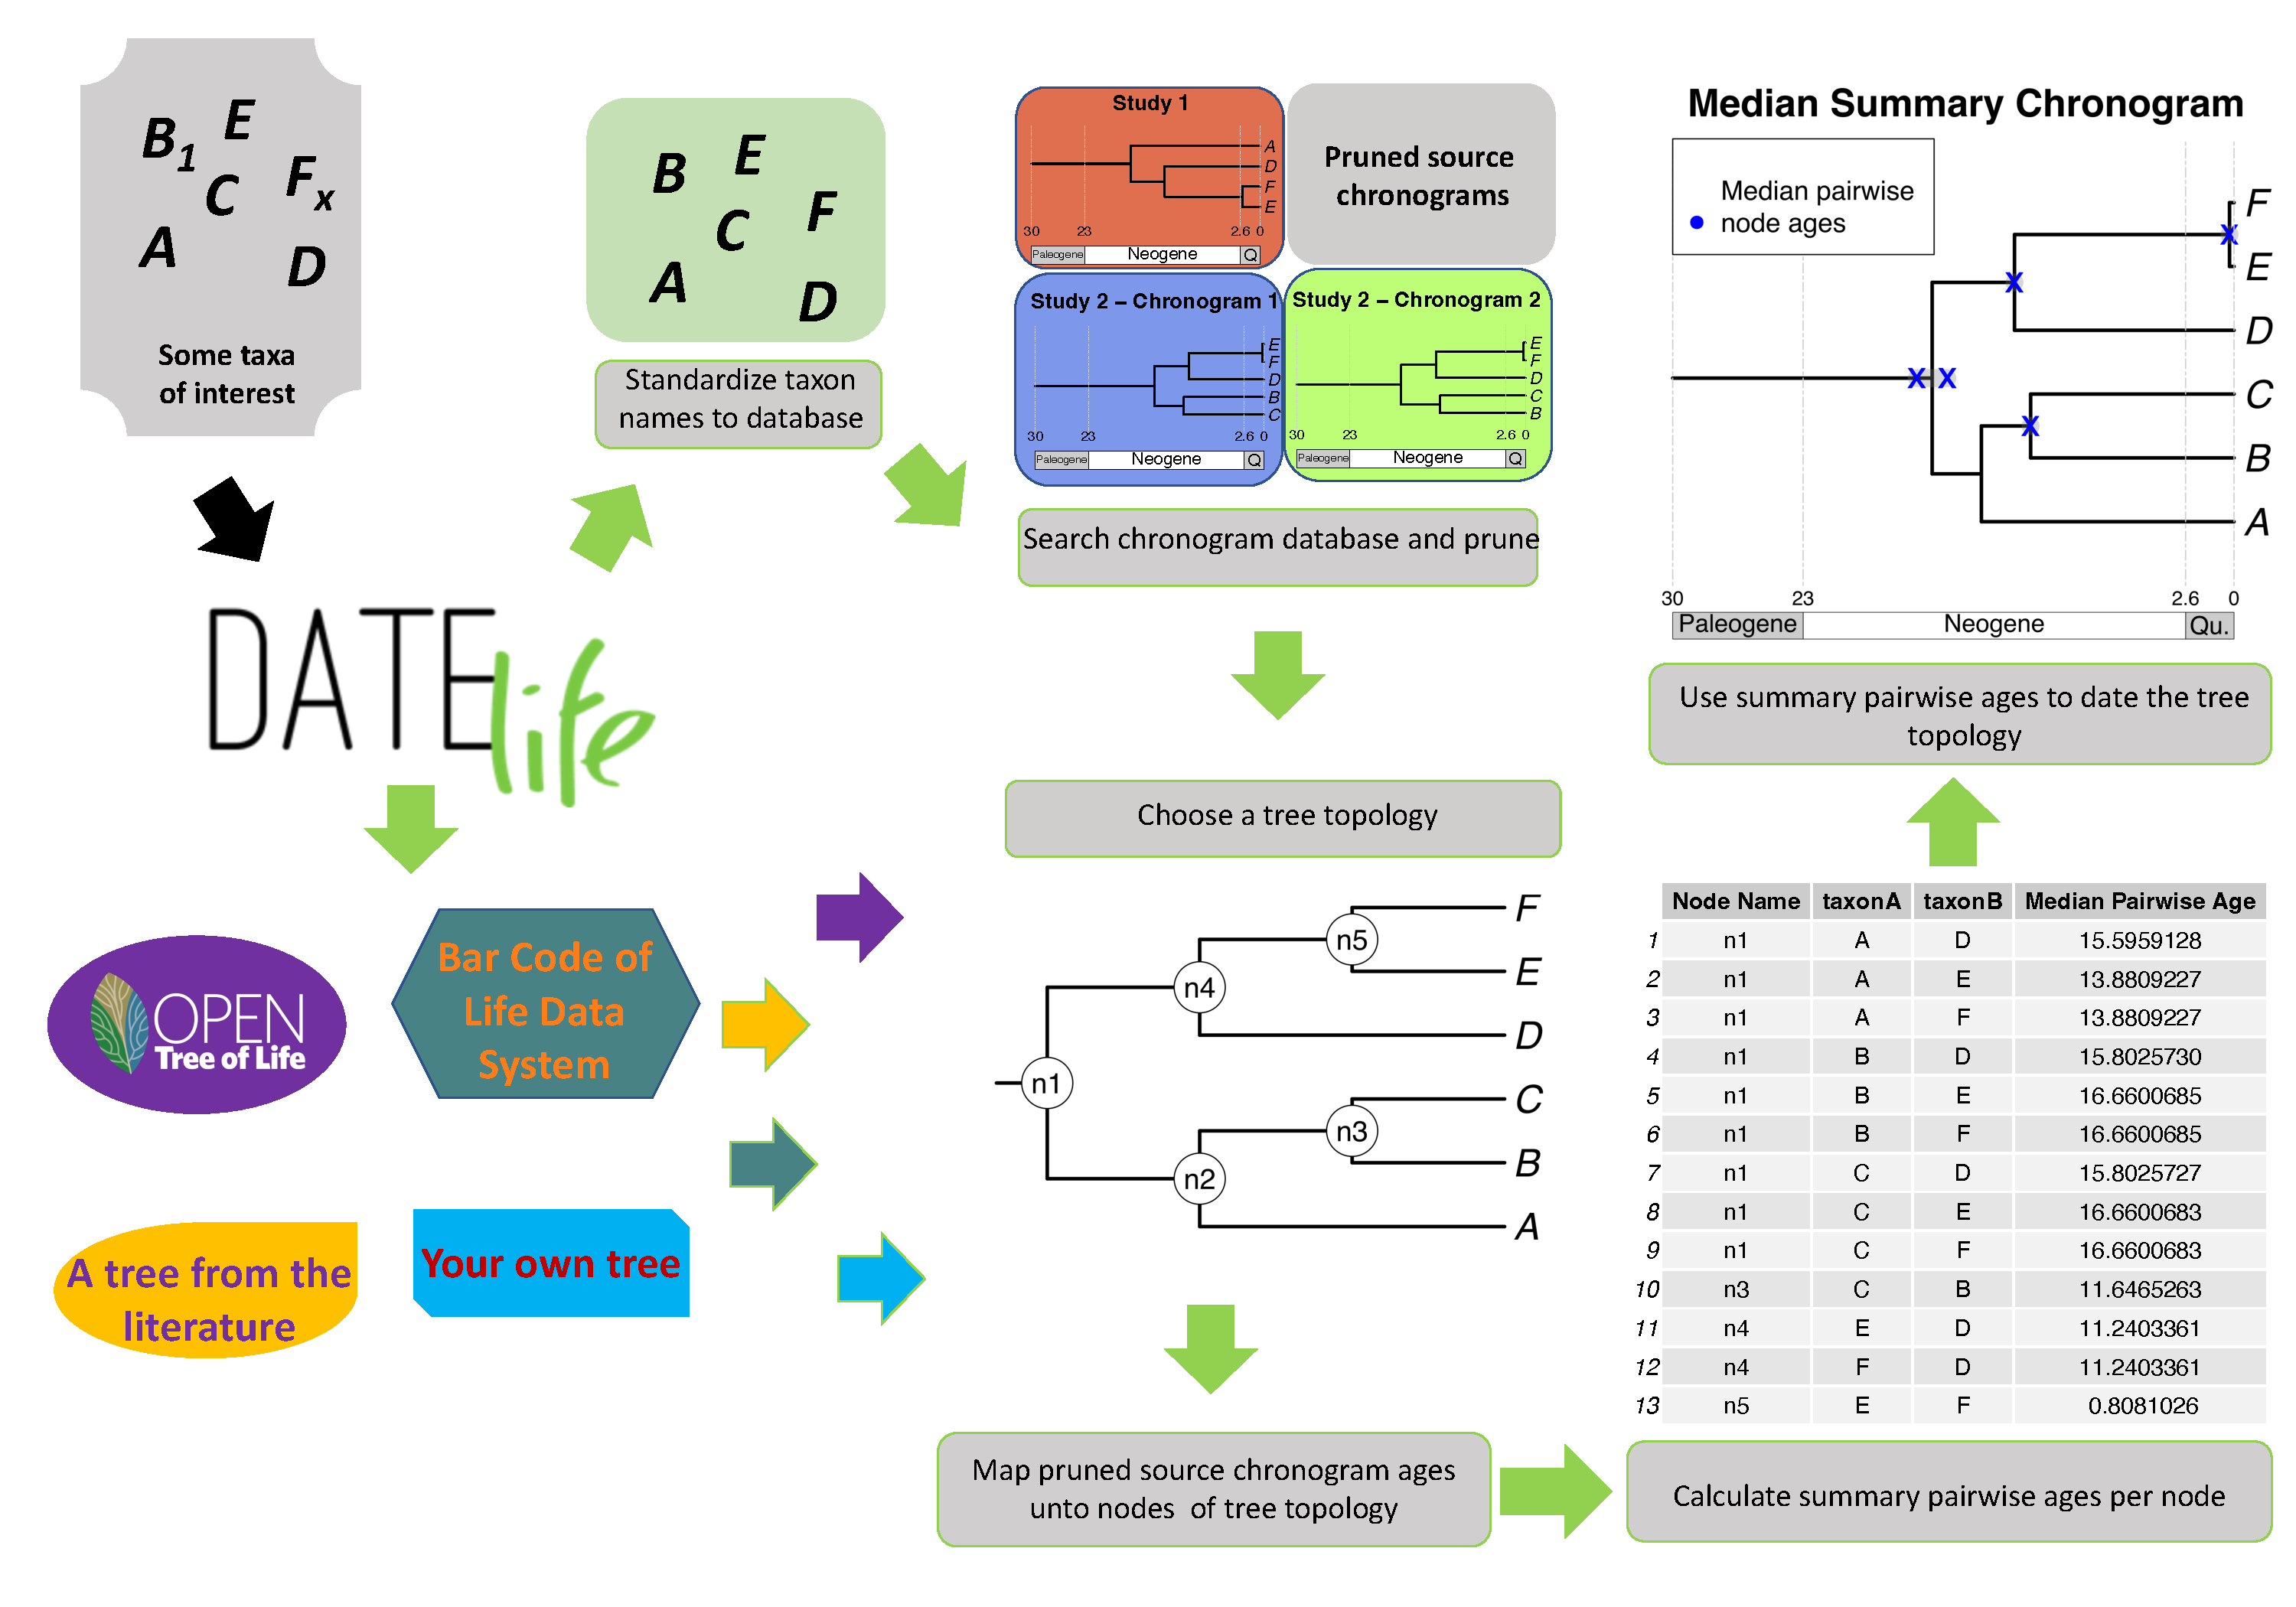
\includegraphics{../figures/figure1/figure1-vertical-final.pdf}
\caption{Stylized DateLife workflow. This shows the general worflows and analyses that can be performed with \texttt{datelife}, via the R package or through the website  at \url{http://www.datelife.org/}. Details on the functions involved on each workflow are shown in \texttt{datelife}'s R package vignette.
}
\label{fig:workflow}
\end{figure}
% \begin{center}
% \textsc{Figure \ref{fig:workflow}}
% \end{center}
\newpage
\begin{figure}[!h]
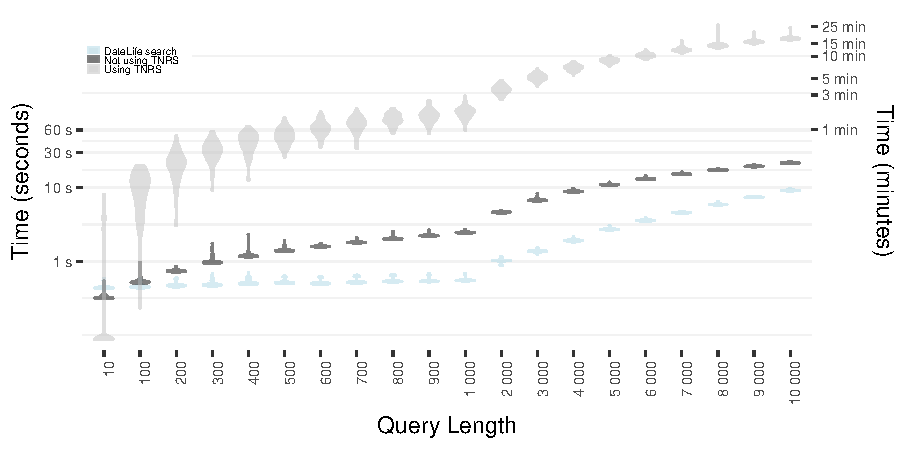
\includegraphics[width=1\linewidth]{../figures/fig_runtime_main.pdf}
\caption{Computation time of query processing and search across \texttt{datelife}'s chronogram database relative to number of input taxon names. We sampled N names from the class Aves for each cohort 100 times and then performed a search with query processing not using the Taxon Names Resoultion Service (TNRS; dark gray), and using TNRS (light gray). We also performed a search using the already processed query for comparison (light blue).}
\label{fig:runtime1}
\end{figure}
% \begin{center}
% \textsc{Figure \ref{fig:benchmark}}
% \end{center}
\newpage
\begin{figure}[!h]
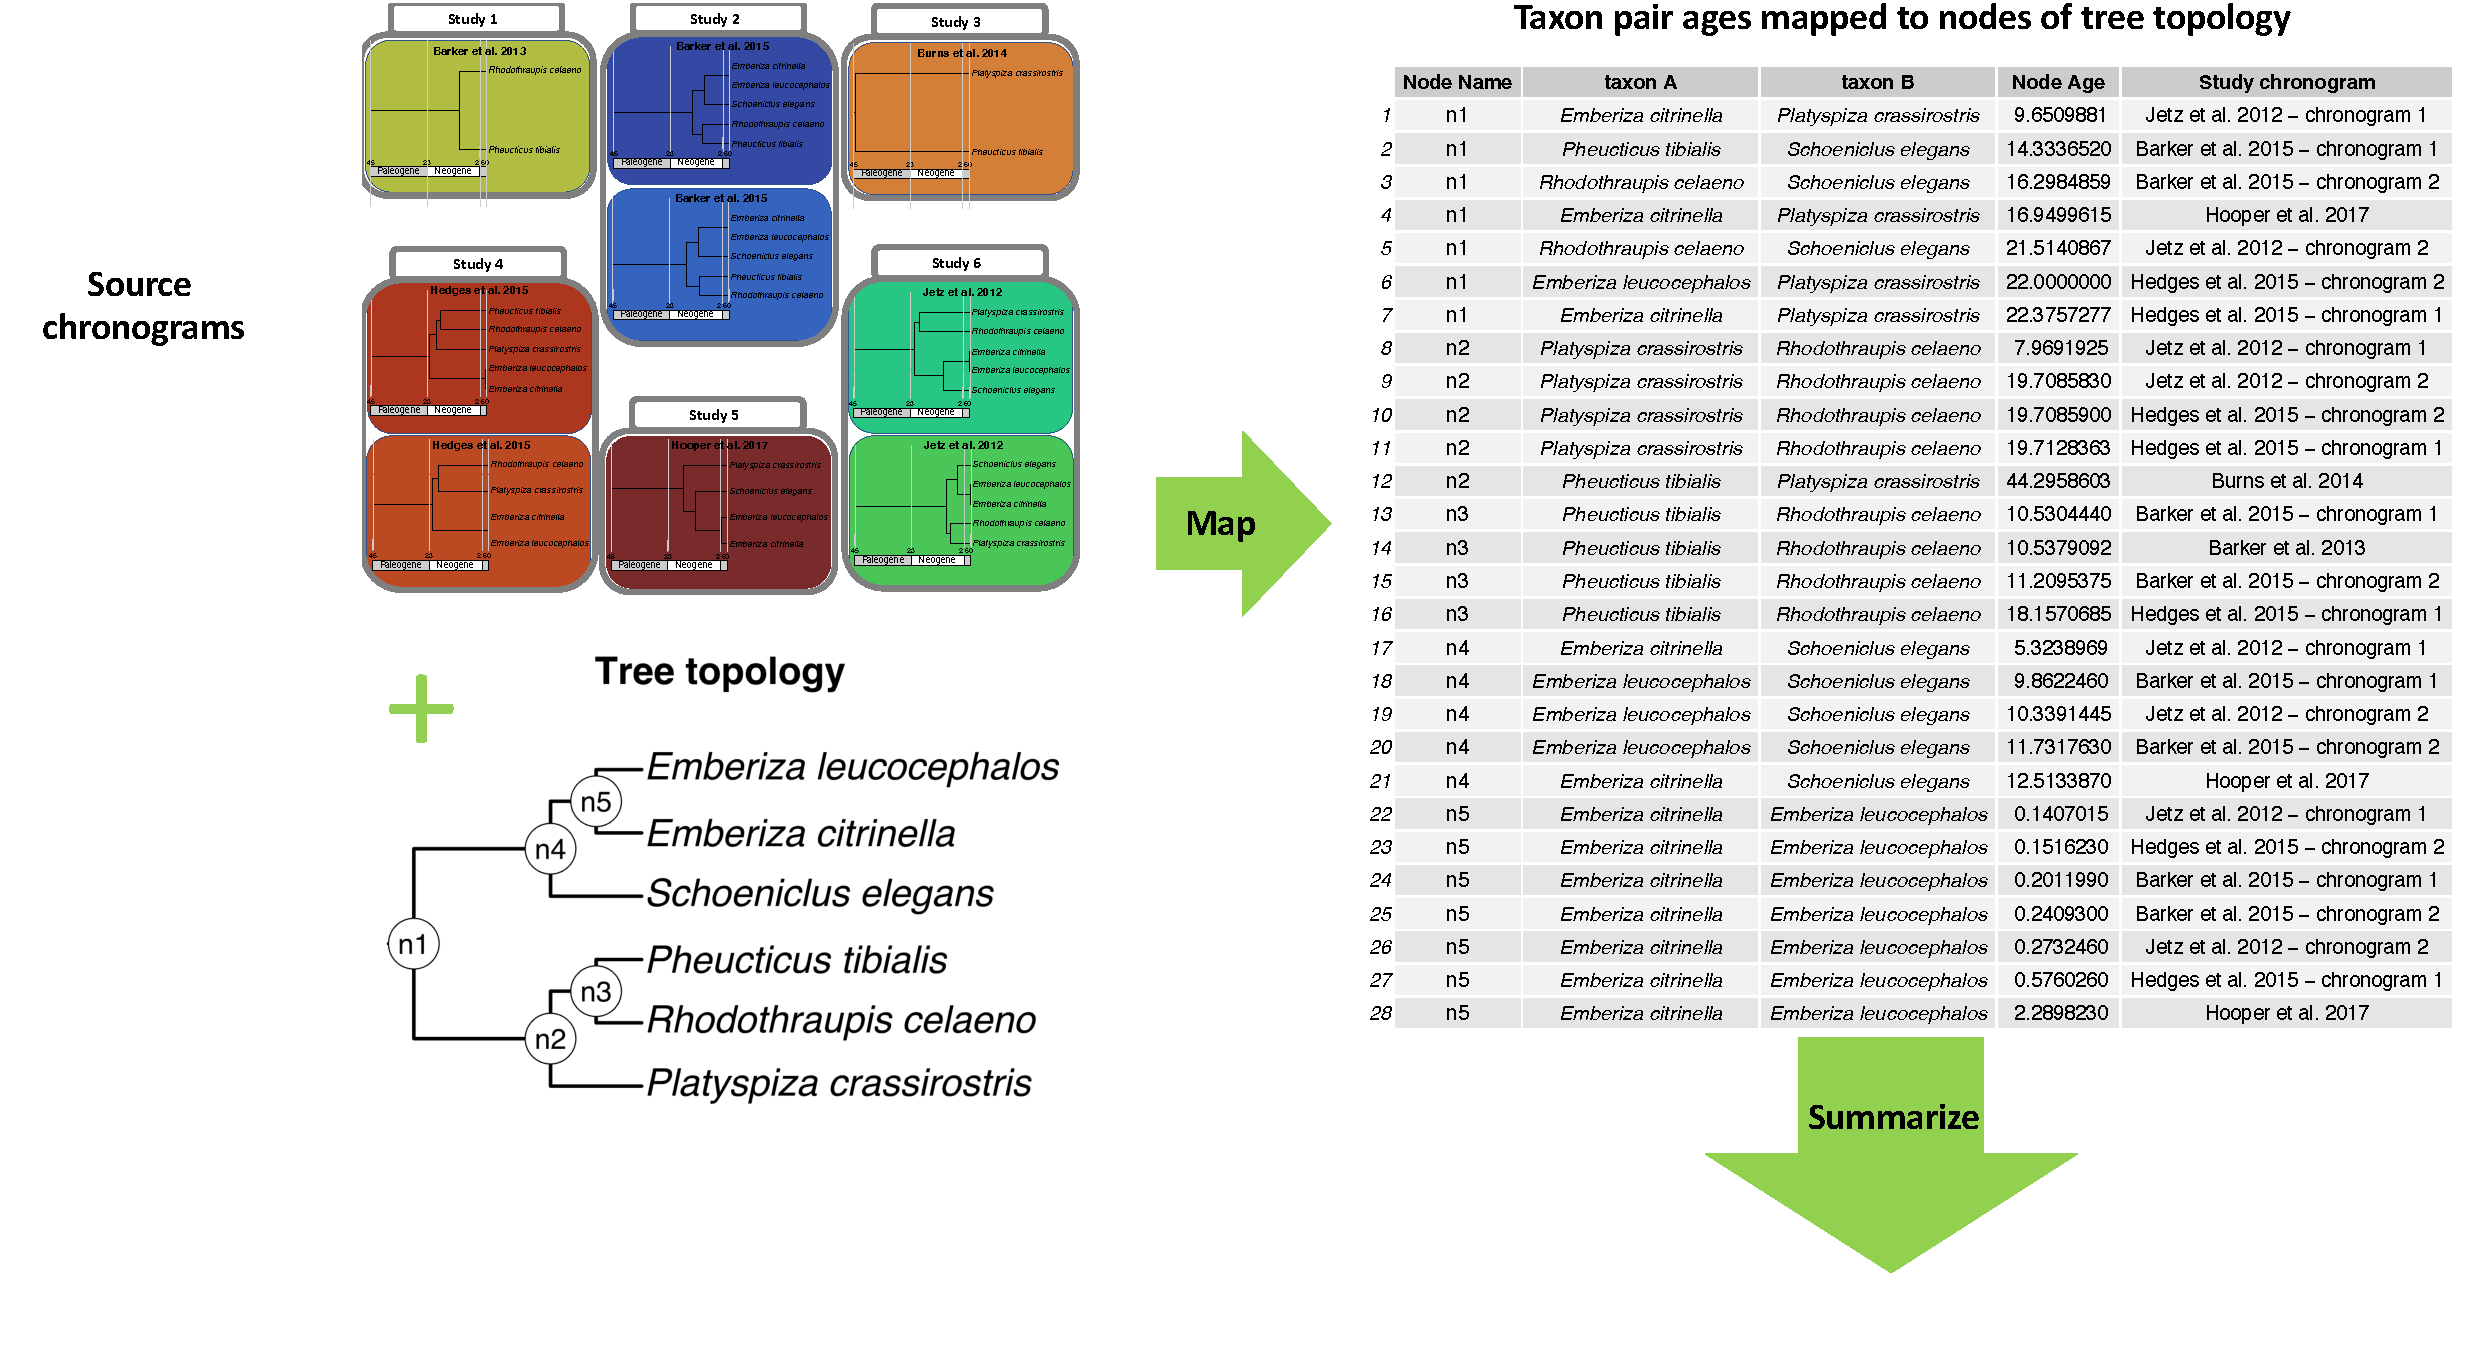
\includegraphics[width=1\linewidth]{../figures/figure2/figure2-1.pdf}
\caption{Age data results of a DateLife search of a small sample of 6 bird species within the Passeriformes. Input names were found across 9 chronograms within 6 independent studies (Barker et al. (\protect\hyperlink{ref-barker2012going}{2012}), Barker et al. (\protect\hyperlink{ref-barker2015new}{2015}), Burns et al. (\protect\hyperlink{ref-burns2014phylogenetics}{2014}), Hedges et al. (\protect\hyperlink{ref-Hedges2015}{2015}), Hooper and Price (\protect\hyperlink{ref-hooper2017chromosomal}{2017}), Jetz et al. (\protect\hyperlink{ref-Jetz2012}{2012}).) This revealed 28 age data points for the queried species names.}
\label{fig:figure2-1}
\end{figure}
% \begin{center}
% \textsc{Figure \ref{fig:figure2-1}}
% \end{center}
\newpage
\begin{figure}[!h]
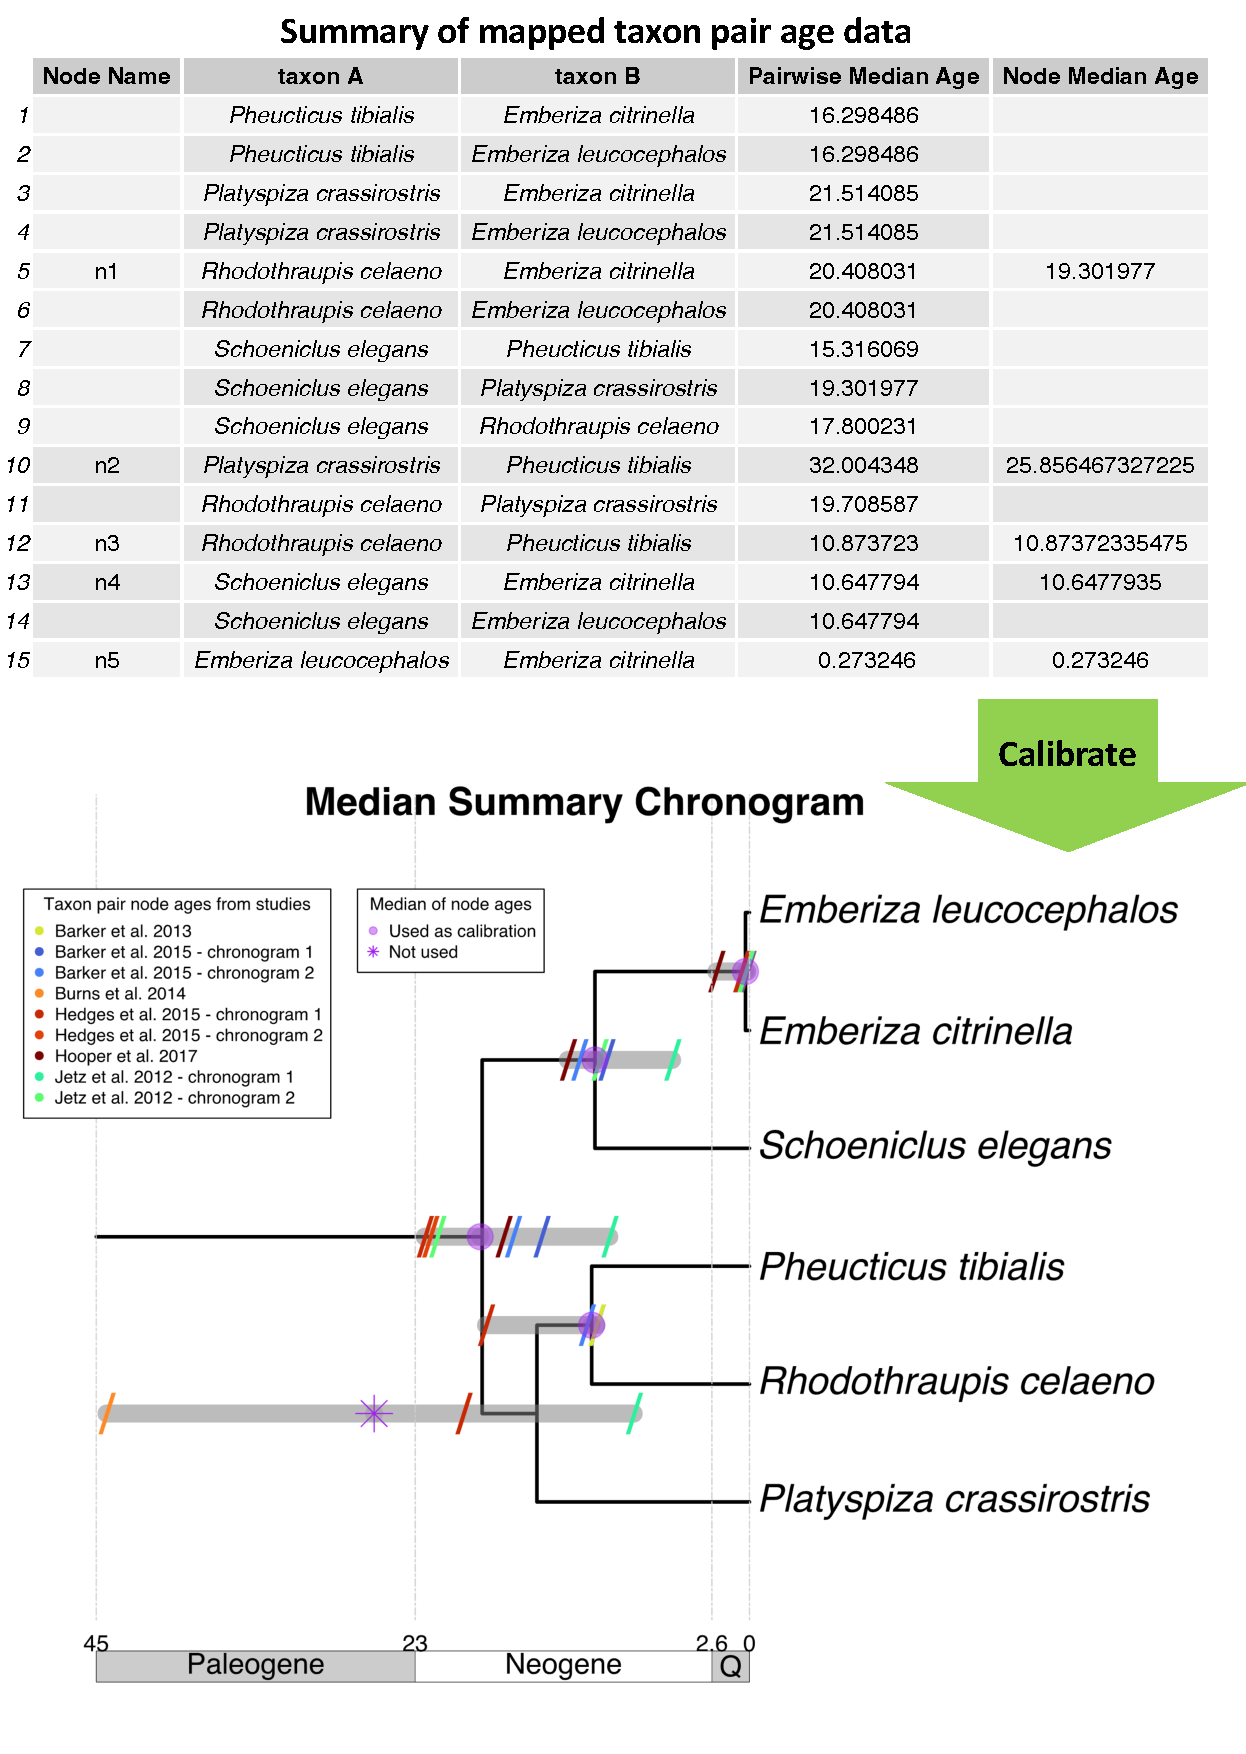
\includegraphics{../figures/figure2/figure2-2.pdf}
\caption{Summarized age data is used as secondary calibrations to date a tree topology as a summary chronogram.}
\label{fig:summaries}
\end{figure}
% \begin{center}
% \textsc{Figure \ref{fig:figure2-2}}
% \end{center}
\newpage
\begin{figure}[!h]
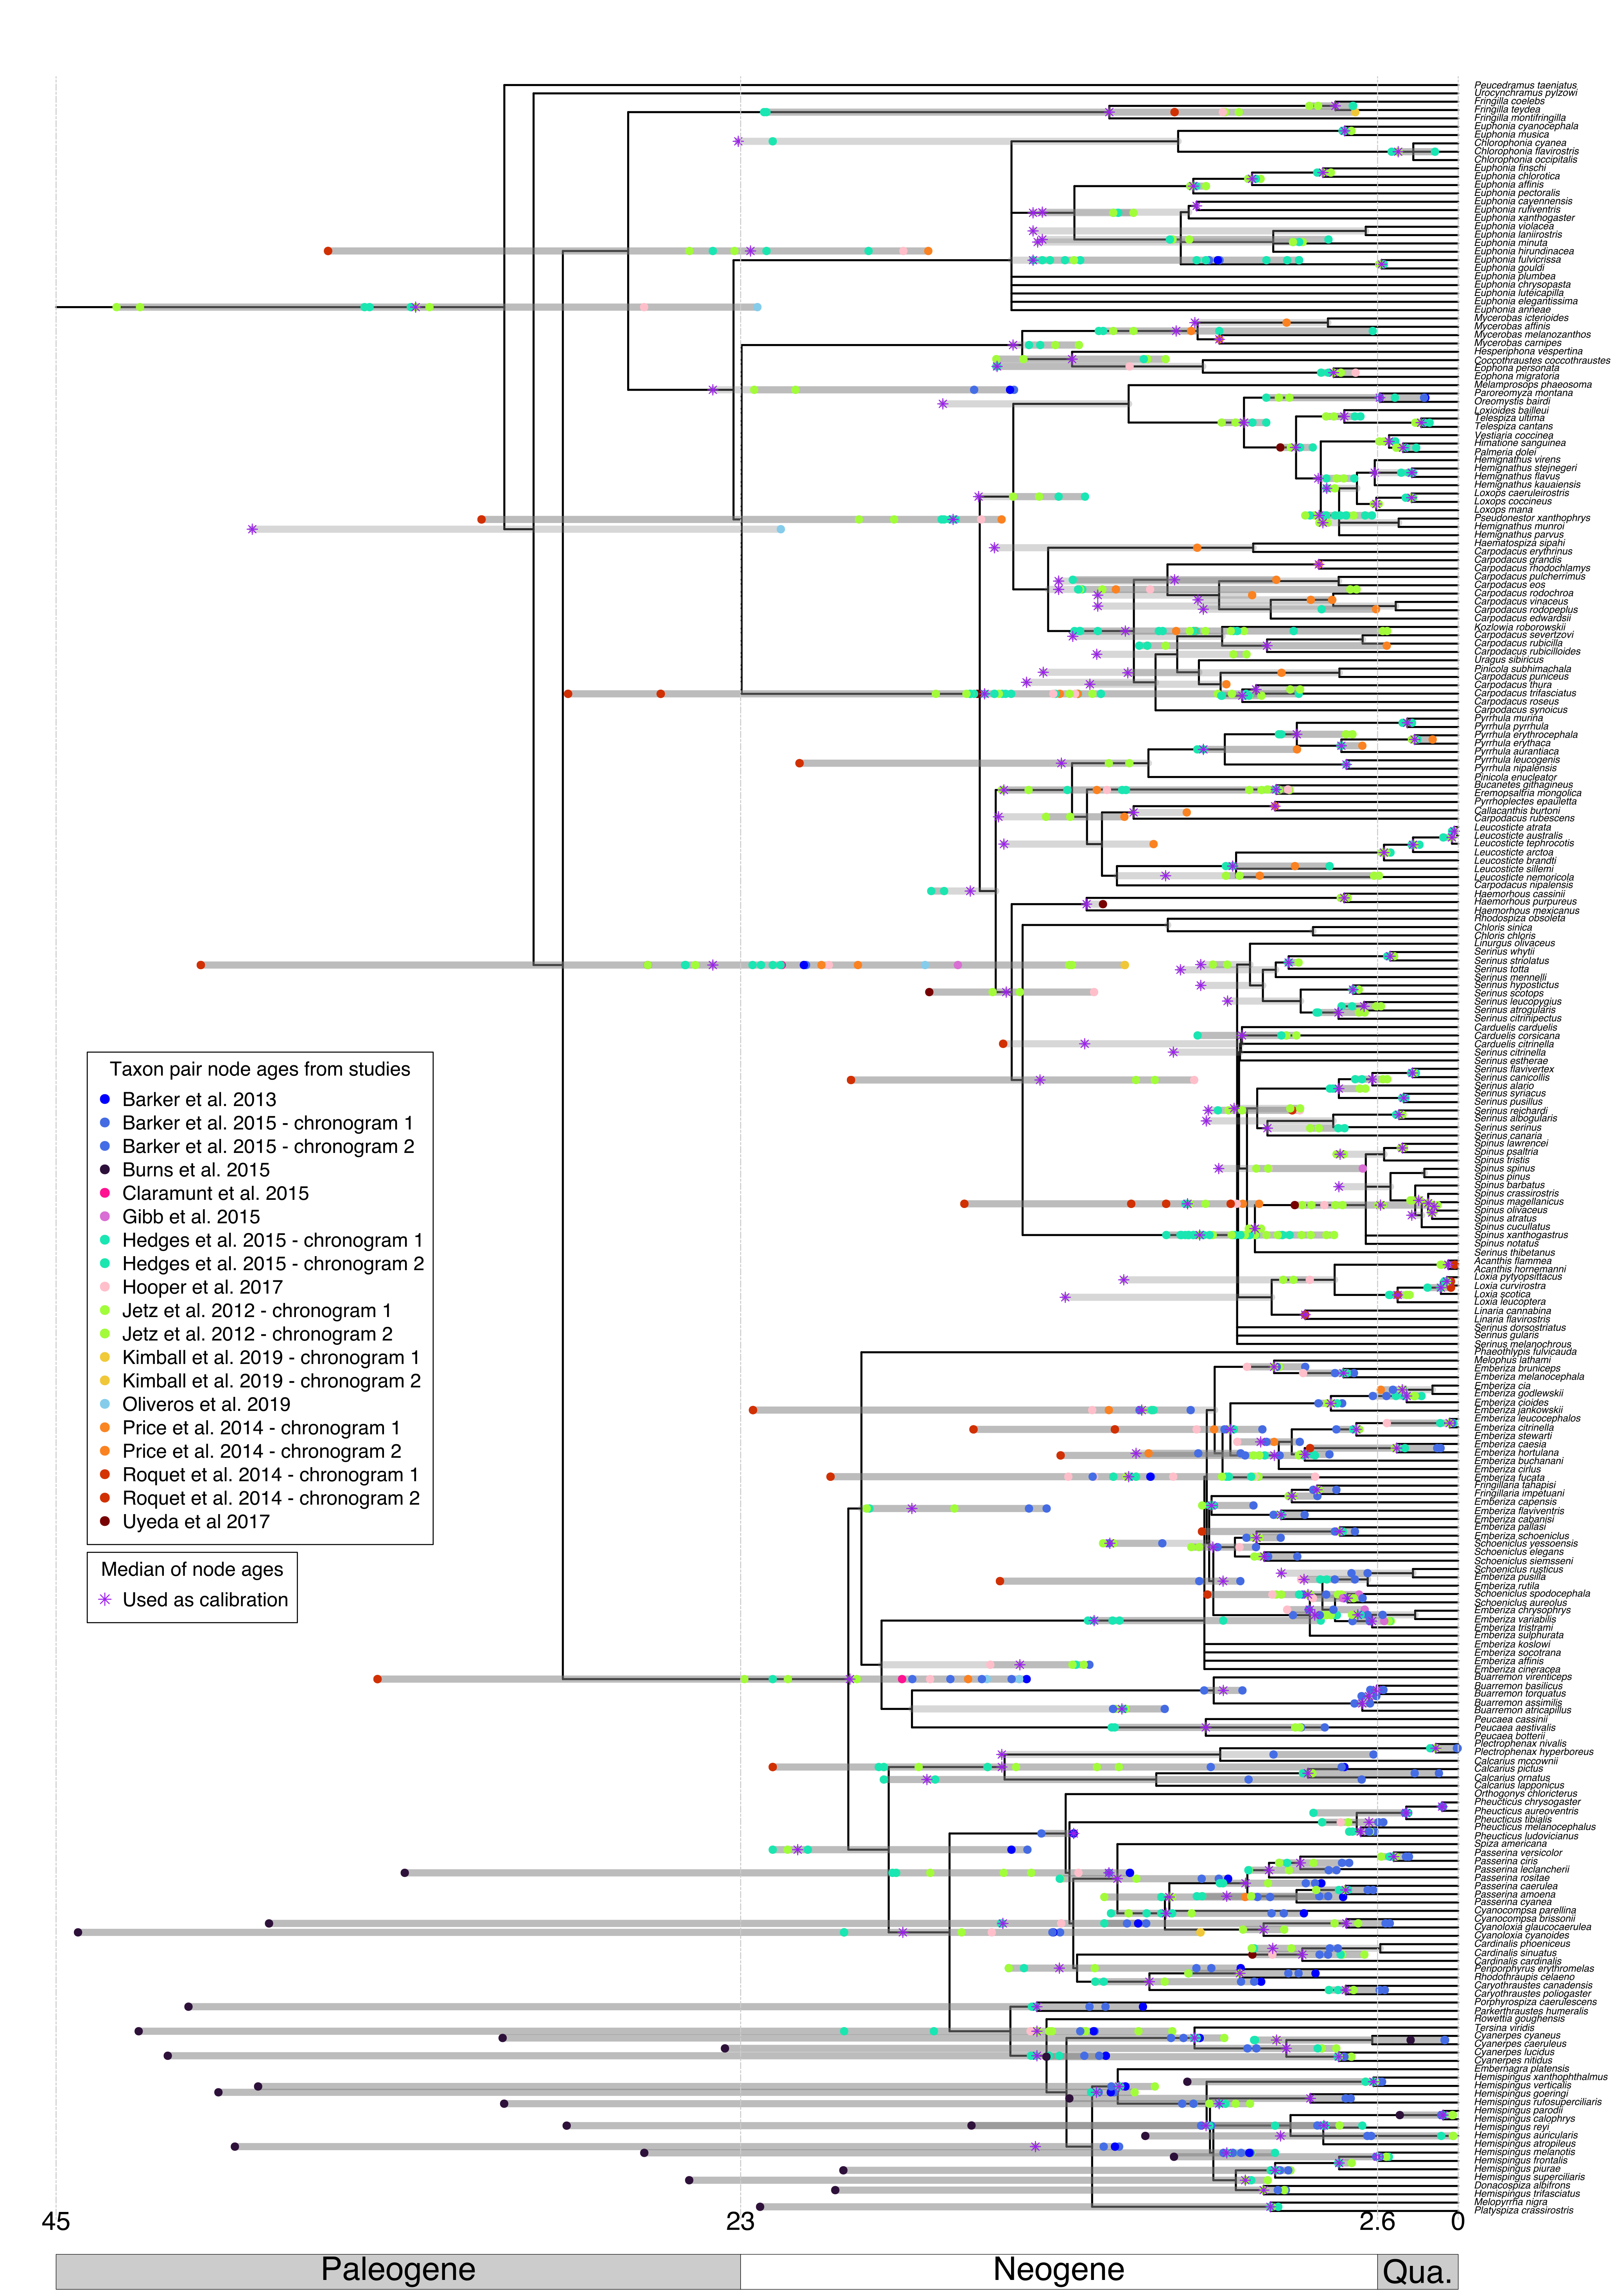
\includegraphics{../figures/figure-fringillidae/median_and_calibration_ages_simple.pdf}
\caption{}
\label{fig:cvbladj}
\end{figure}
% \begin{center}
% \textsc{Figure \ref{fig:fringillidages}}
% \end{center}
\newpage
\begin{figure}[!h]
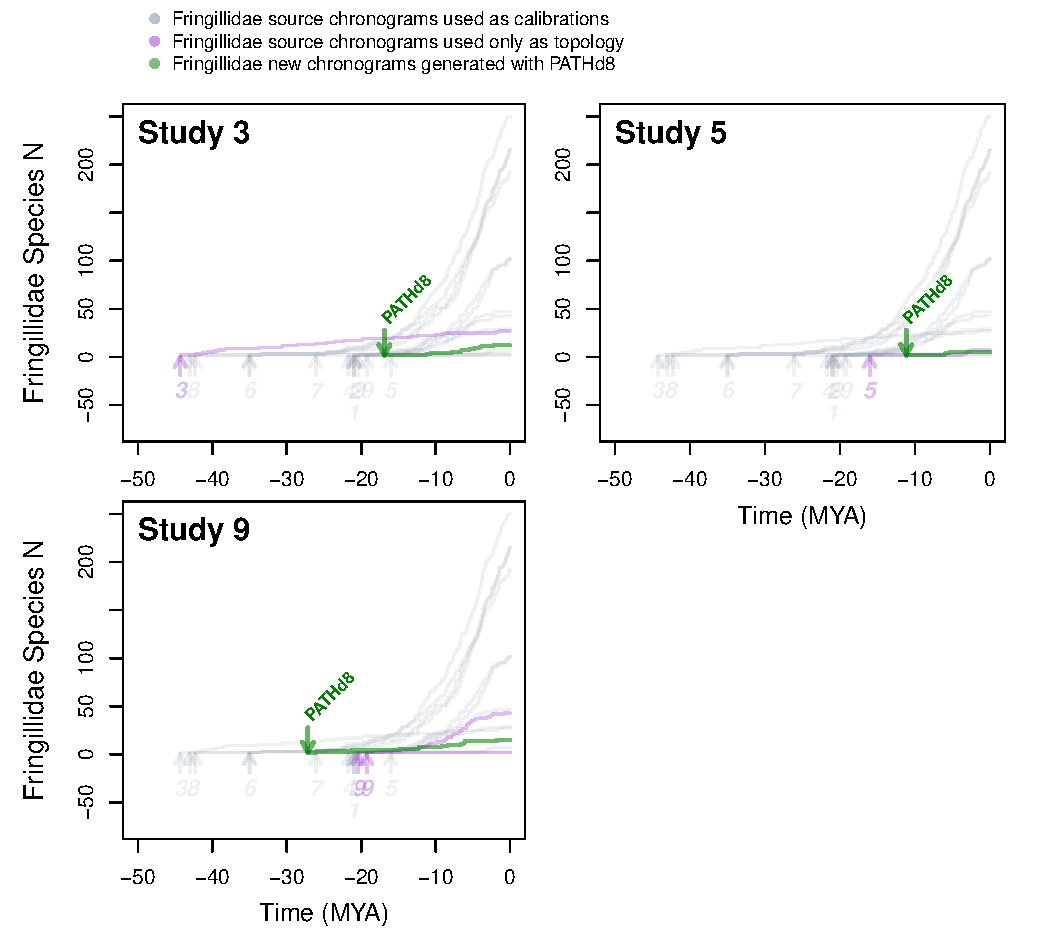
\includegraphics{../figures/fig_crossval_boldsumm.pdf}
\caption{}
\label{fig:cvbold}
\end{figure}
% \begin{center}
% \textsc{Figure \ref{fig:cvbold}}
% \end{center}
LTT plots showing results from the cross-validation analyses of trees with branch length reconstructed with data from the Barcode of Life Database (BOLD) dated using PATHd8. We could construct a tree with branch lengths for all source chronograms. However, dating with PATHd8 was only successful in three source chronograms shown here.

% \end{linenumbers}
